\documentclass[11pt]{article}
\usepackage{amsmath, amssymb, amsfonts,  graphicx, enumerate, float, wrapfig}
\usepackage[margin=0.5in]{geometry}
\graphicspath{{./}}
\newcommand*{\vs}{\vspace{1cm}}
\newcommand*{\next}{\noindent}
\newcommand*{\set}{\setcounter{equation}{0}}


\title{Notes - 3.6 A Summary of Curve Sketching}
\author{Juan J. Moreno Santos}
\date{October 2023}

\begin{document}
\maketitle

So far, we have reviewed the following characteristic of a function in each of the following sections:\\
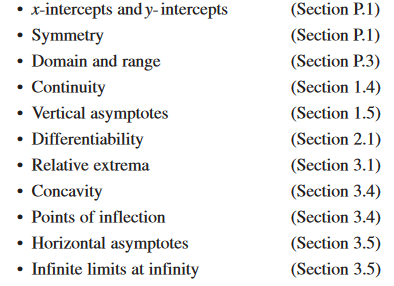
\includegraphics{1.png}\\

\section{Guidelines for analyzing the graph of a function.}
\begin{enumerate}
    \item Determine the domain and range of the function.
    \item Determine the intercepts, asymptotes, and symmetry of the graph.
    \item Locate the x-values for which $f'(x)$ and $f''(x)$ either are zero or do not exist. Use those results to determine relative extrema and inflection points.
\end{enumerate}

\section{Examples}
\subsection{Sketching the graph of a rational function}
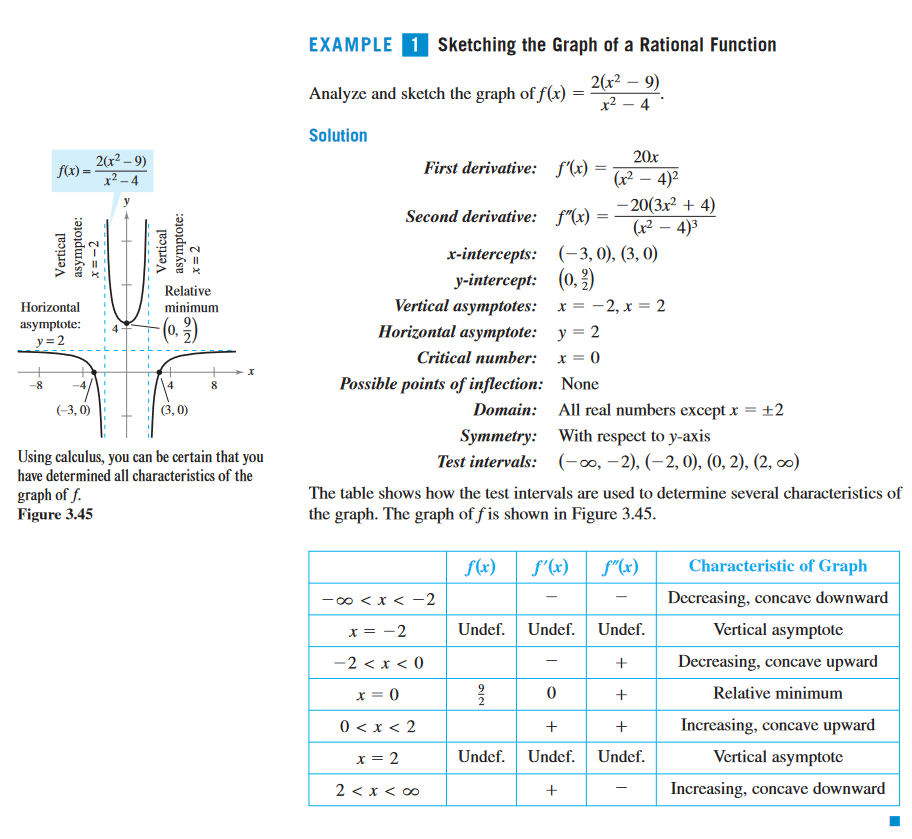
\includegraphics{2.png} \newpage
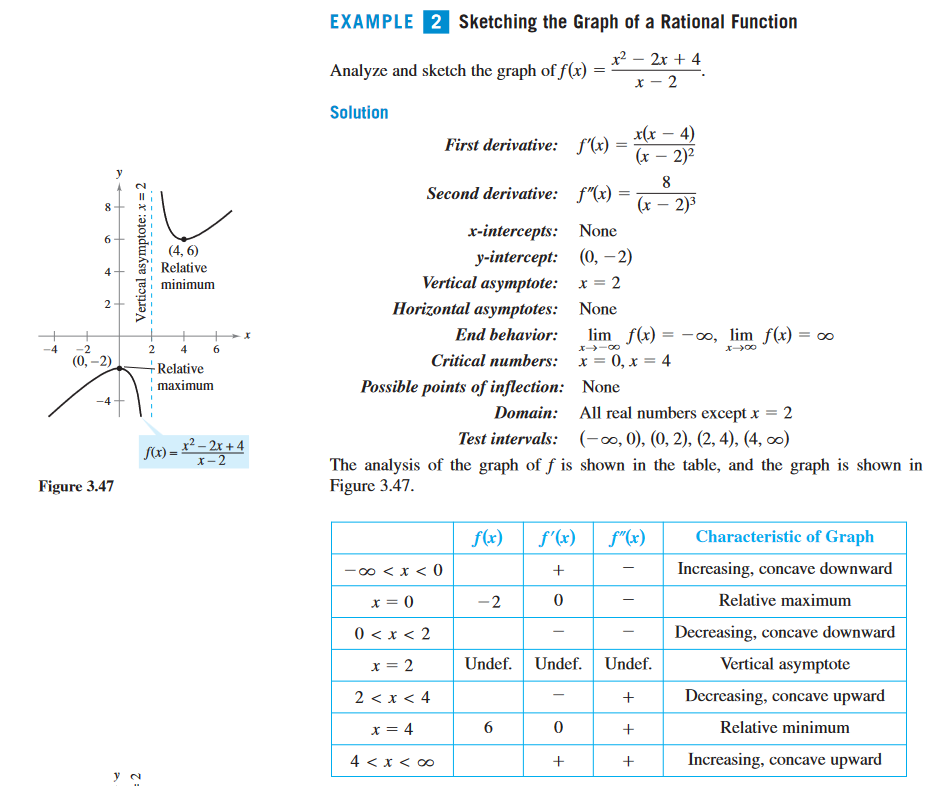
\includegraphics{3.png} \newpage
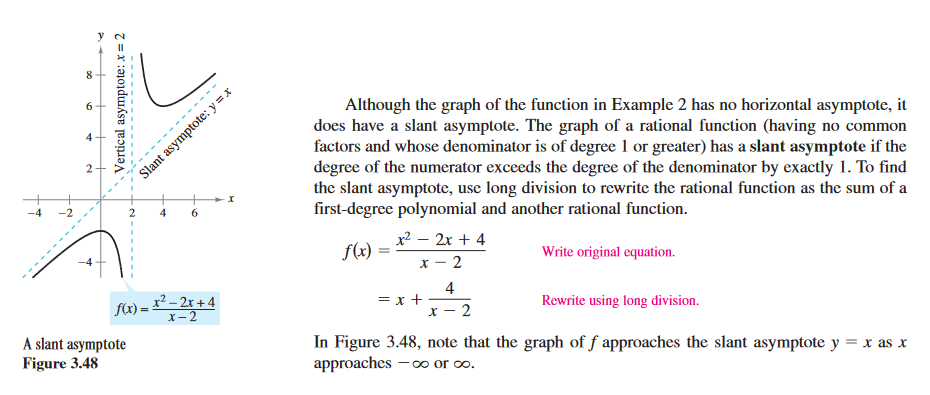
\includegraphics{4.png}

\subsection{Sketching the graph of a radical function}
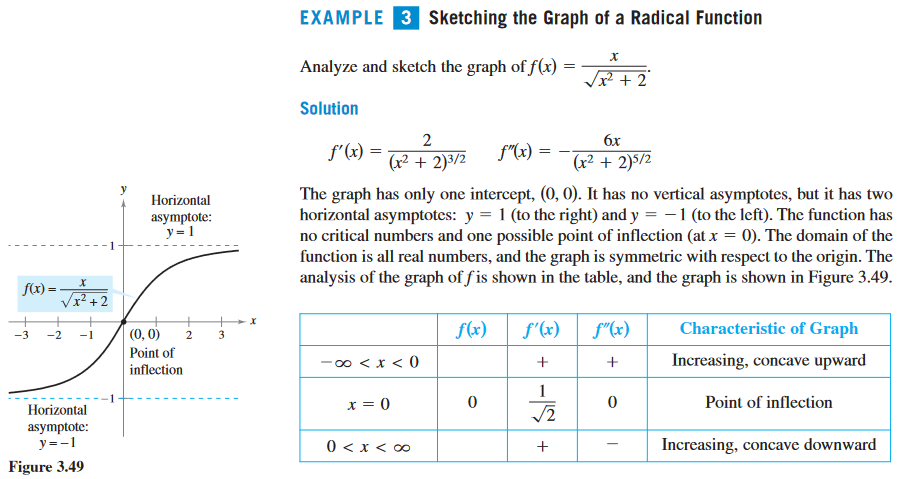
\includegraphics{5.png} \newpage
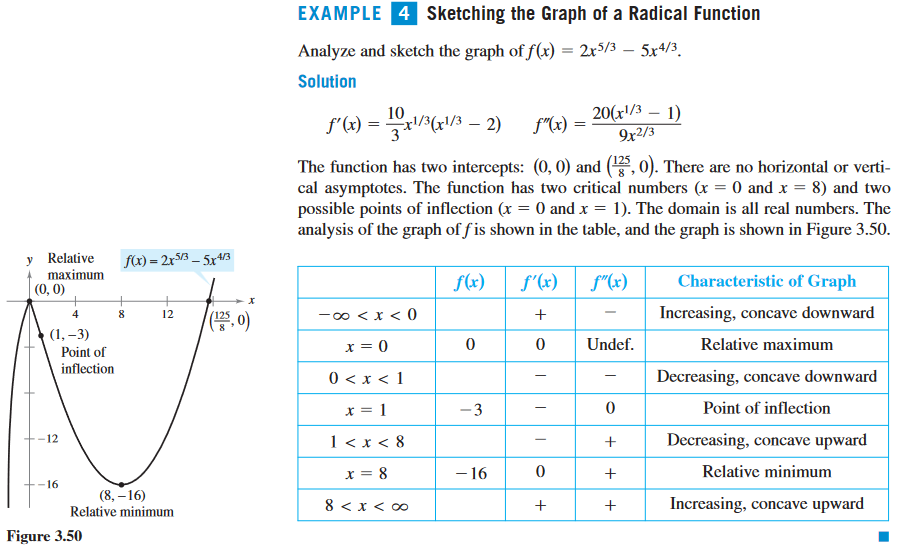
\includegraphics{6.png}

\subsection{Sketching the graph of a polynomial function}
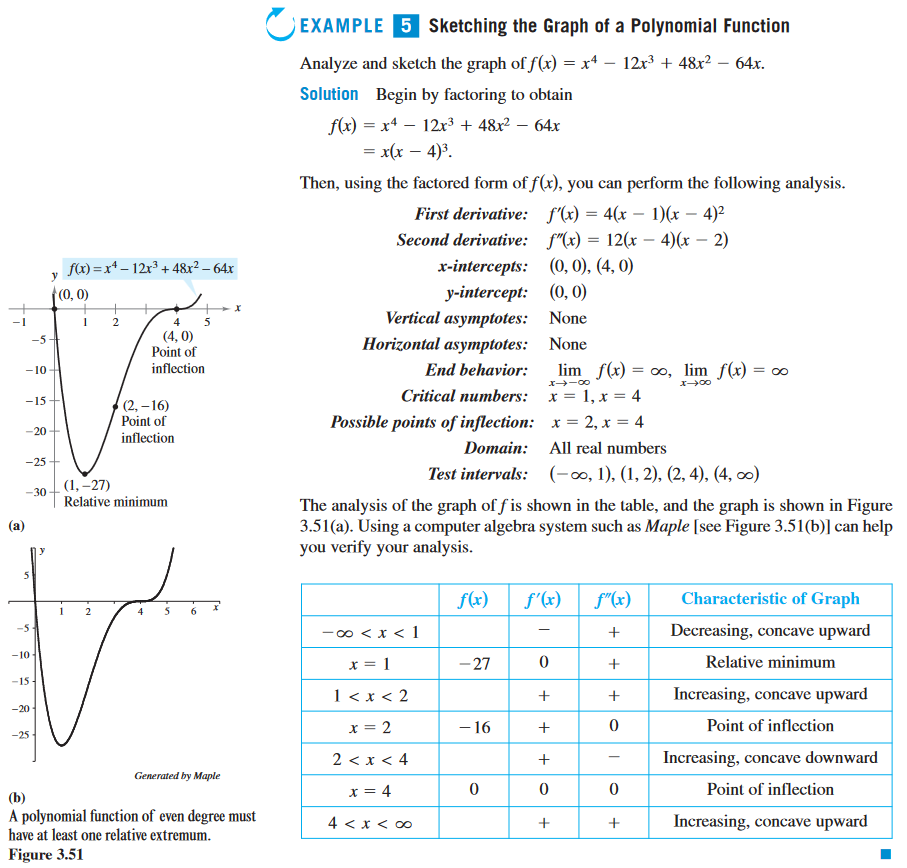
\includegraphics{7.png}

\subsection{}










\end{document}